\chapter{Test Cases and convergence tests}\label{ChapAppendTestCases}

%%%%%%%%%%%%%%%%%%%%%%%%%%%%%%%%%%%%%%%%%%%%%%%%%%%%%%%%%%%%%%%%%%%%%%%%%%%%%%%
%\section{Difference tests: make check}
%\subsection{Test 1: Advection}
%\clearpage
%\subsection{Test 2: Diffusion}
%\clearpage
%\subsection{Test 3: Source/Fall-model/vertical grid}
%\subsubsection{3.1 Line source / Wilson-Huang / constant dz}
%\subsubsection{3.2 point source / No fall (tracer) / constant dz}
%\subsubsection{3.3 point source / Wilson-Huang / constant dz}
%\subsubsection{3.4 point source / Ganser / constant dz}
%\subsubsection{3.5 point source / Stokes+slip / constant dz}
%\subsubsection{3.6 profile source / Wilson-Huang / constant dz}
%\subsubsection{3.7 line source / Wilson-Huang / constant dz}
%\subsubsection{3.8 point source / Wilson-Huang / piecewise linear dz}
%\subsubsection{3.9 point source / Wilson-Huang / constant log(dz)}
%\subsubsection{3.10 point source / Wilson-Huang / custom dz}
%\clearpage
%\subsection{Test 4: }
%\subsubsection{4.1 Umbrella\_air}
%\subsubsection{4.2 Suzuki k=4, GSD with Aggr.}
%\subsubsection{4.3 Umbrella}
%\subsubsection{4.4 Suzuki k=4, 1-grain, Global domain}
%
%\clearpage
%\section{Unit testing of functions}
%\subsection{Atmosphere.f90}
%\subsubsection{Dens\_IdealGasLaw}
%\subsubsection{Visc\_Sutherland}
%\subsubsection{lambda\_MeanFreePath}
%\subsection{Tephra.f90}
%\subsubsection{vset\_WH}
%\subsubsection{vset\_WH\_slip}
%\subsubsection{vset\_WH\_PCM}
%\subsubsection{vset\_Gans}
%\subsubsection{vset\_Stokes\_slip}
%
\clearpage
\section{Convergence Tests}\label{ApxTestSecConv}

\subsection{Test case 1: Horizontal advection of smooth source}
\clearpage
\subsection{Test case 2: Vertical advection of smooth source}
\clearpage
\subsection{Test case 3: Horizontal rotational advection of 2-D cone and box}
This test case examines the effect of rigid-body rotation of a concentration profile
through one revolution.  The concentration profile is given below for a Cartesian grid
and consists of a cone centered at $x=-0.45$, $y=0$ and a box located at
$0.1<x<0.6$, $-0.25<y<0.25$.
%  \begin{linenomath*}
\begin{eqnarray}\label{EqTC3Source}
q_0 &=& \left\{ \begin{array} {l@{\quad \quad}l}
1         &:  \mathrm{if}\,\,\, 0.1 < x < 0.6 \,\,\mathrm{and}\\
          &  \,\,\, -0.25 < y < 0.25 \\
1-r/0.35  &:  \mathrm{if}\,\,\, r < 0.35 \\
0         &: \mathrm{Otherwise}
\end{array}
\right.
\end{eqnarray}
%  \end{linenomath*}
where $r \equiv \sqrt{\left( x+0.45\right)^2+y^2}$.
The wind field is given by
%  \begin{linenomath*}
\begin{eqnarray}
u(x,y)=2y & & v(x,y)=-2x \label{EqTC3Wind}
\end{eqnarray}
%  \end{linenomath*}

\clearpage
\subsection{Test case 4: 1-D diffusion}
\clearpage
\subsection{Test case 5: Reversable horizontal shearing}
To evaluate the ability of these numerical schemes to track advection in highly
deforming wind fields, a test was run using a transient, rotational wind field
where the rotational velocity about the pole
($\phi_0=0^{\circ}$, $\lambda_0=0^{\circ}$) is given by (shown in figure b)
%  \begin{linenomath*}
\begin{equation}\label{EqTC5Wind}
\omega(\phi,\lambda) = -0.5\sin(d\pi/18) \cos(\pi t/4)
\end{equation}
%  \end{linenomath*}
where $d$ is the angular distance (in degrees) of $\phi$, $\lambda$ from $\phi_0$, $\lambda_0$.
The initial concentration distribution (shown in figure a) is given by
%  \begin{linenomath*}
\begin{equation}\label{EqTC5Source1}
q(\lambda,\phi,z,t=0)=0.5 (1.0+\cos(\pi r))
\end{equation}
%  \end{linenomath*}
where $r$ is given by:
%  \begin{linenomath*}
\begin{eqnarray}
r &=& \sqrt{(\phi+16.0)^2 + \lambda^2/16} \label{EqTC5Source2} \\
r &=& \mathrm{min(}1.0,r) \label{EqTC5Source3}
\end{eqnarray}
%  \end{linenomath*}
The initial concentration distribution is deformed into a long strand at $t=2$ (figure c),
then the deformation reverses back to the initial configuration.  A similar test in
Cartesian coordinates %\citep[Sec. 5.7.4]{Durran99} 
was also conducted.  Versions of the
test cases for both Cartesian and spherical coordinates are shown.

Figure shows the behavior of the various numerical methods for this test problem at $t=4$
when the deformation should return to zero.  Each plot of figure should be compared with
figure a.  Since diffusion is not calculated in this test problem, any distortion of the
final profile is a result of numerical diffusion.  The CTU method without the use of a
limiter recovers the initial profile with the greatest fidelity.  However it is possible
in this case, since the use of limiters is non-linear, that errors in the advection in
the clock-wise rotation are simply reversed in the counter-clock-wise phase of the oscillation.

\clearpage
\subsection{Test case 6: Method of manufactured solutions}
In addition to the two test cases shown above (rotational advection and reversible
rotational shear) simple 1-dimensional advection and 1-dimensional diffusion tests
were conducted along the coordinate axis to verify convergence properties.  Simple
tests such as these are useful for identifying obvious bugs in the code; however,
they do not fully test all aspects of the algorithm.  In general, analytic solutions
are not available for the advection-diffusion-sedimentation equation in a non-trivial
wind field with realistic pressure and temperature profiles (See \cite{Stockie11} for
solutions in simplified atmospheric conditions.).  However, the Method of Manufactured
Solutions (MMS) %\citep{Roache09,Salari00}
provides some guidance on how to generate
analytic solutions for non-trivial atmospheric conditions which will invoke all
components of the algorithm, all terms of the governing equation and boundary conditions.
This will allow us to confirm the order of accuracy of the complete algorithm.

If a domain is specified and atmospheric and boundary conditions prescribed, then a
``source" (a transient spatial distribution of tephra characterizing the eruption)
results in a ``solution" (a transient spatial distribution of airborne and deposited
tephra) through the governing equation.  In Eq. \ref{EqGovEqVect}, the source is $S$
and the solution is $q$.  In general, we do not know the solution {\it a priori} that
is the result of the source term and boundary conditions.  The idea behind the Method
of Manufactured Solutions is to find a compatible set of functions for the source and
the solution by specifying $q$ and solving for $S$.

To employ the MMS method, we first choose a model geometry (domain and topography) and
define the physical state ($p$, $T$, $u$, $v$, $w$, $\mathbf{K}$).  Next, we simply
choose a non-trivial solution, $q$, ideally one with a 3-dimensional, transient structure
that is easily differentiable.  This artificial solution need not be physically realistic
since our goal is to evaluate the performance of the algorithm, not model a particular
physical process.  This solution can be inserted into the governing equation
(Eq. \ref{EqGovEqVect}) and evaluated to generate a non-trivial, three-dimensional, transient
source term, $S$.  Note that this source term will not resemble the vertical distribution
described in section \ref{SubSecDepo}, but instead will be a transient three-dimensional
function.  Initial conditions are generated by simply evaluating the chosen solution at
$t=t_0$.  Boundary conditions can be determined by evaluating $q$ along the boundary.
Applying the algorithm with these initial and boundary conditions, along with the source
term, will generate a numerical solution that can be compared with the solution that was
initially chosen.  Grid convergence studies of this test case will quantify the order of
accuracy of the full algorithm.

We use the following domain for the MMS test.
$-100<x<100\, \mathrm{km}$, $-100<y<100\, \mathrm{km}$, $0<z<20 \, \mathrm{km}$.
We use a standard atmosphere for the pressure and temperature profiles given by
%\citet[chap. 1]{Wallace77}
:  $P = P_0 \exp (-z/\delta)$ and $T = T_0 + \theta z$.
For the wind velocity structure, we adopt a horizontal model to mimic wind shear with small
vertical perturbations:
$u = U_0$, $v = V_0/2\left( 1 + \tanh ( z-Z_0)\right)$,
$w=-W_0 \cos(\pi x/\lambda_{xy})\cos(\pi y/\lambda_{xy})$.
The diffusivity is set to a constant.
The fall model is set via the equations of section \ref{SubSecDepo} using the ideal gas
law and Sutherland's Law to calculate $\rho_a$ and $\eta_a$.

The solution we choose is given below.
%  \begin{linenomath*}
\begin{equation} \label{EqMMSSolution}
q = Q_0 \, \mathrm{sech} \left( \frac{x}{\lambda_{xy}}\right) \mathrm{sech} \left( \frac{y}{\lambda_{xy}}\right)
\mathrm{sech} \left( \frac{z}{\zeta}\right)
\end{equation}
%  \end{linenomath*}
where $\zeta=W_0 t + \zeta_0$.
To calculate the source term, $S$, we need to calculate the first partial derivatives of $q$
with respect to $t$, and both first and second partial derivatives with respect to the
spatial coordinates.
%  \begin{linenomath*}
\begin{eqnarray}
\frac{\partial q}{\partial t} &=& q\left[ z \frac{W_0}{\zeta^2} \mathrm{tanh}(z/\zeta)\right] \label{EqMMSQt} \\
\frac{\partial q}{\partial x} &=& q\left[ -\frac{\tanh (x/\lambda_{xy})}{\lambda_{xy}} \right] \label{EqMMSQx} \\
\frac{\partial^2 q}{\partial x^2} &=& q\left[ \frac{\tanh^2 (x/\lambda_{xy})}{\lambda^2_{xy}} - \frac{\mathrm{sech}^2 (x/\lambda_{xy})}{\lambda^2_{xy}}\right]  \label{EqMMSQxx} \\
%\frac{\partial q}{\partial y} &=& q\left[ -\frac{\tanh (y/\lambda_{xy})}{\lambda_{xy}} \right] \\ \label{EqMMSQy}
%\frac{\partial^2 q}{\partial y^2} &=& q\left[ \frac{\tanh^2 (y/\lambda_{xy})}{\lambda^2_{xy}} - \frac{\mathrm{sech}^2 (y/\lambda_{xy})}{\lambda^2_{xy}}\right] \\ \label{EqMMSQyy}
\frac{\partial q}{\partial z} &=& q \left[ - \frac{\mathrm{tanh}(z/\zeta)}{\zeta}\right]\\ \label{EqMMSQz}
\frac{\partial^2 q}{\partial z^2} &=& q \left[ \frac{1}{\zeta^2}\left( \mathrm{tanh}^2(z/\zeta) - \mathrm{sech}^2(z/\zeta)\right)\right] \label{EqMMSQzz}
\end{eqnarray}
%  \end{linenomath*}
The equations for first and second derivatives in $y$ are of the same form as
Eq.s \ref{EqMMSQx} and \ref{EqMMSQxx}.
The choice of Eq. \ref{EqMMSSolution} is not unique, but is guided by the simple form of
the derivatives in Eq.s \ref{EqMMSQt}--\ref{EqMMSQzz}.  An arbitrarily complex form of
$q$ can be chosen, as determining $S$ is straight-forward once the derivatives are
calculated; although it may be more cumbersome to implement. Assembling these terms into
the governing equation (Eq. \ref{EqGovEqVect}) leads to a simple expression for the source
term, $S$, which is a continuous function of space and time.  By selecting individual
constants (i.e. $U_0$, $V_0$, $W_0$, $Z_0$, $\zeta_0$) we can selectively activate or
deactivate branches of the algorithm.  If all are activated, we have an analytic solution
against which we can compare the full advection-diffusion-sedimentation equation.  This is
particularly important for calculating splitting errors due to the decomposition of the
governing equation via the method of fractional steps. The constants used in the testcase
are given in Table \ref{TabMMSConsts}.

$L_1$-norm convergence results are shown in figure \ref{FigMMSConverge}.  The full
simulation using the semi-Lagrangian scheme for the horizontal advection produce results
that converge with an order accuracy of 1.5.
Without the use of limiters, the DCU and CTU schemes converge with second-order accuracy.
With MinMod, SuperBee and MC limiters, the accuracy of the calculations with DCU and CTU
for horizontal advection reduces to approximately order 1.8.  The fact that these
convergence rates are nearly second-order suggests that splitting errors are minimal.
Although the use of limiters in this particular case reduces the order of convergence
slightly, they significantly improve the resolution of sharp boundaries.

\clearpage
\section{Validation Testing}
\subsection{Spurr (Deposit): August 19, 1992}
\begin{figure}[htbp]
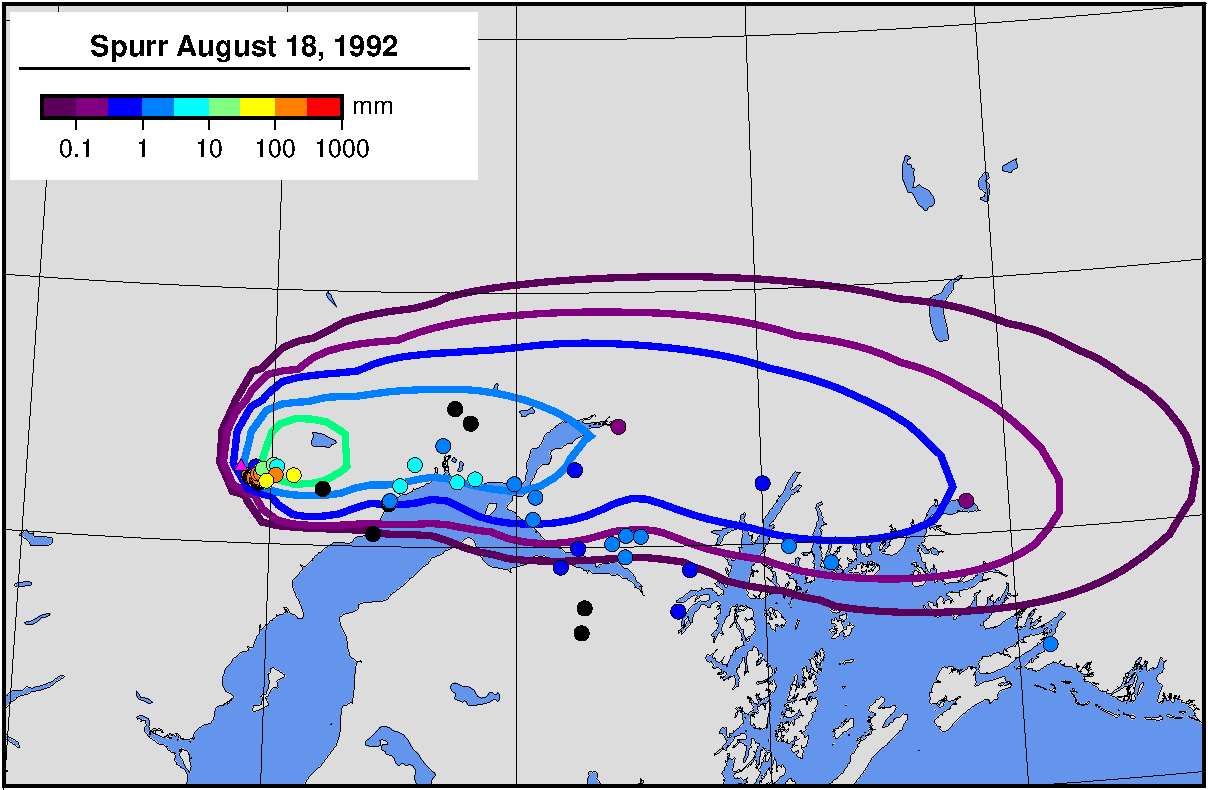
\includegraphics[angle=0,scale=0.6]{Figures/TestCase_Results/ValidTest/Spurr_Deposit.pdf}
\parbox{15cm}{\caption{\label{FigTestValSpurr} Deposit}}
\end{figure}

\clearpage
\subsection{Mt. St. Helens (Deposit with Aggregates): May 18, 1980}
\begin{figure}[htbp]
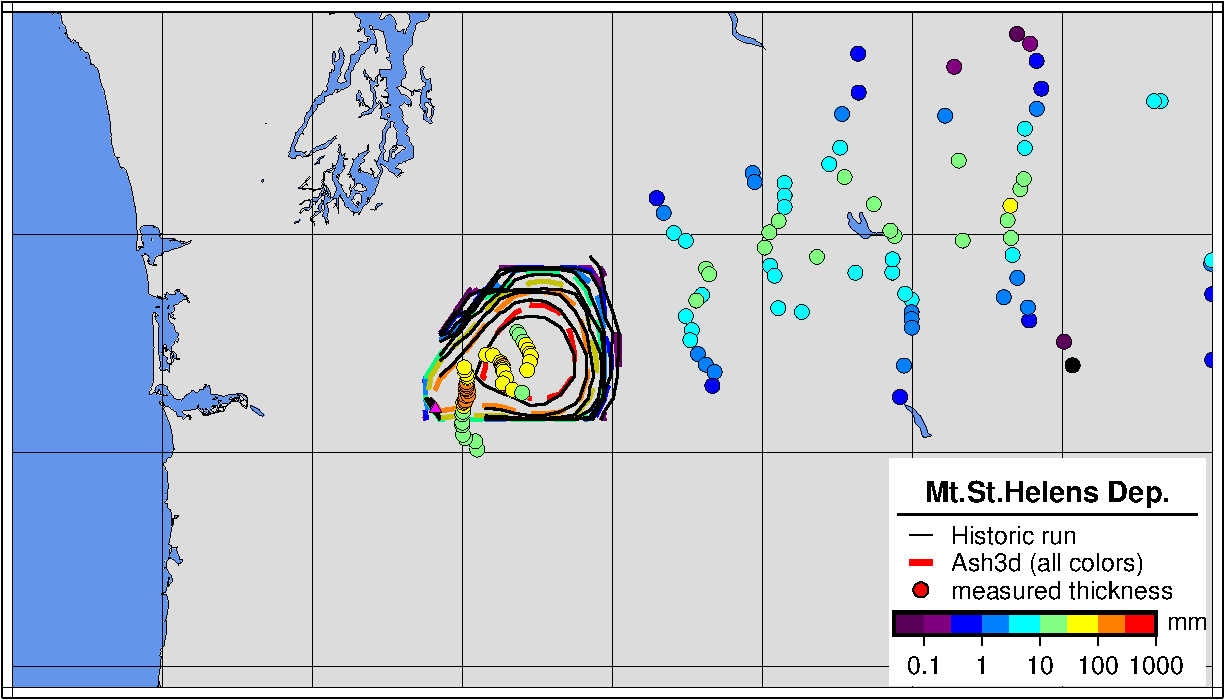
\includegraphics[angle=0,scale=0.6]{Figures/TestCase_Results/ValidTest/MSH_Deposit.pdf}
\parbox{15cm}{\caption{\label{FigTestValMSH} Deposit}}
\end{figure}

\clearpage
\subsection{Kasatochi (Ash cloud load): August 8, 2008}
\begin{figure}[htbp]
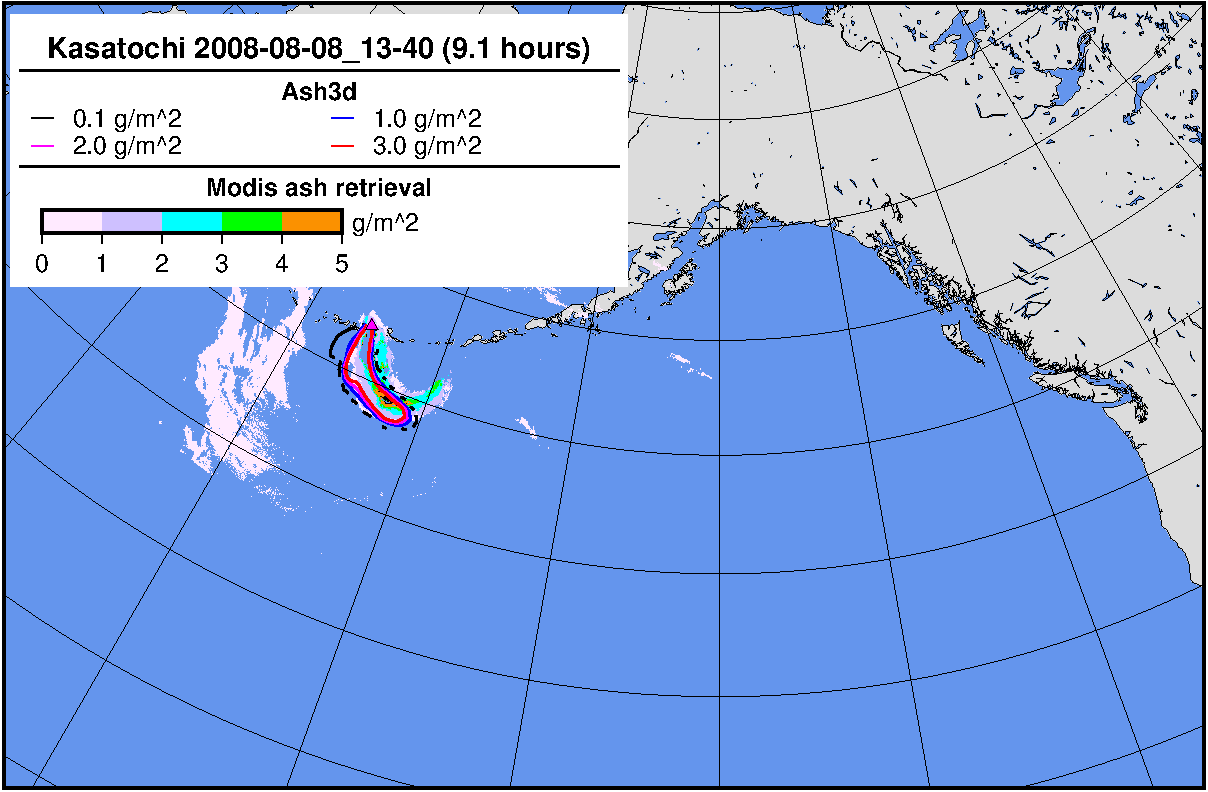
\includegraphics[angle=0,scale=0.3]{Figures/TestCase_Results/ValidTest/Kasatochi_CloudLoad_0.pdf}
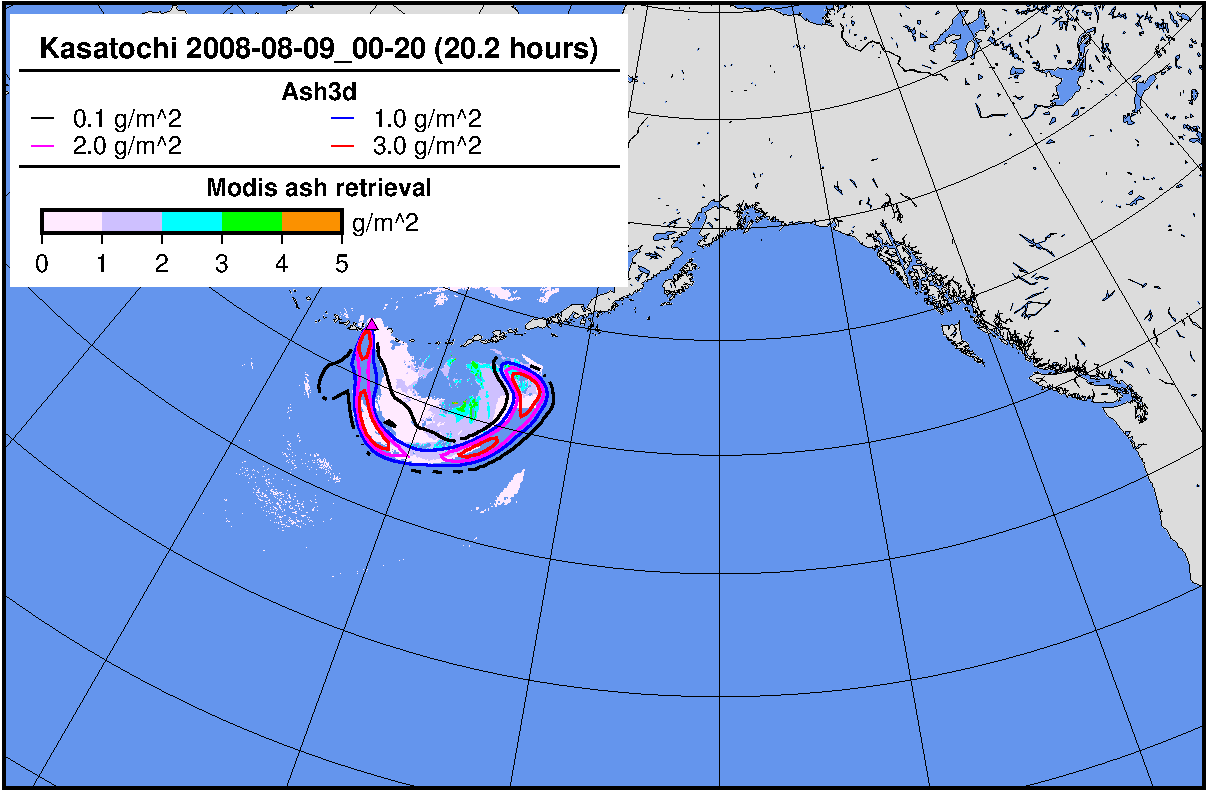
\includegraphics[angle=0,scale=0.3]{Figures/TestCase_Results/ValidTest/Kasatochi_CloudLoad_1.pdf}
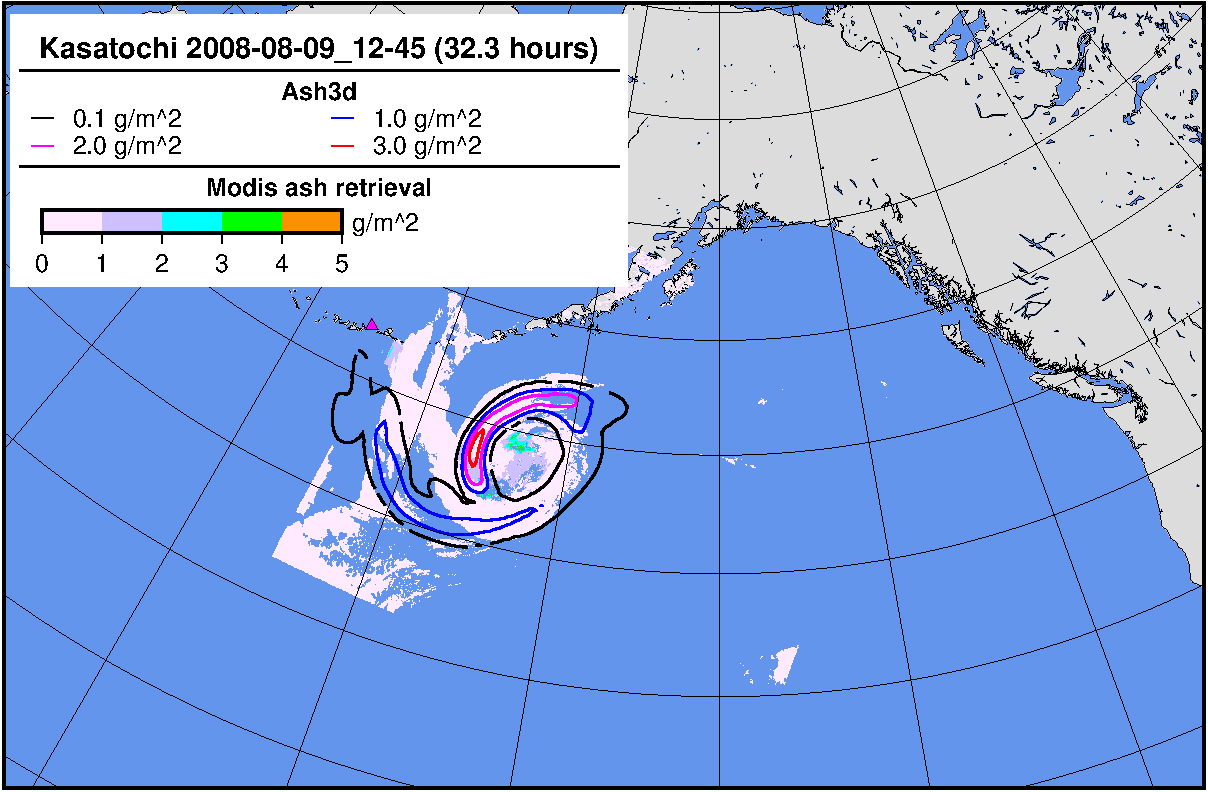
\includegraphics[angle=0,scale=0.3]{Figures/TestCase_Results/ValidTest/Kasatochi_CloudLoad_2.pdf}
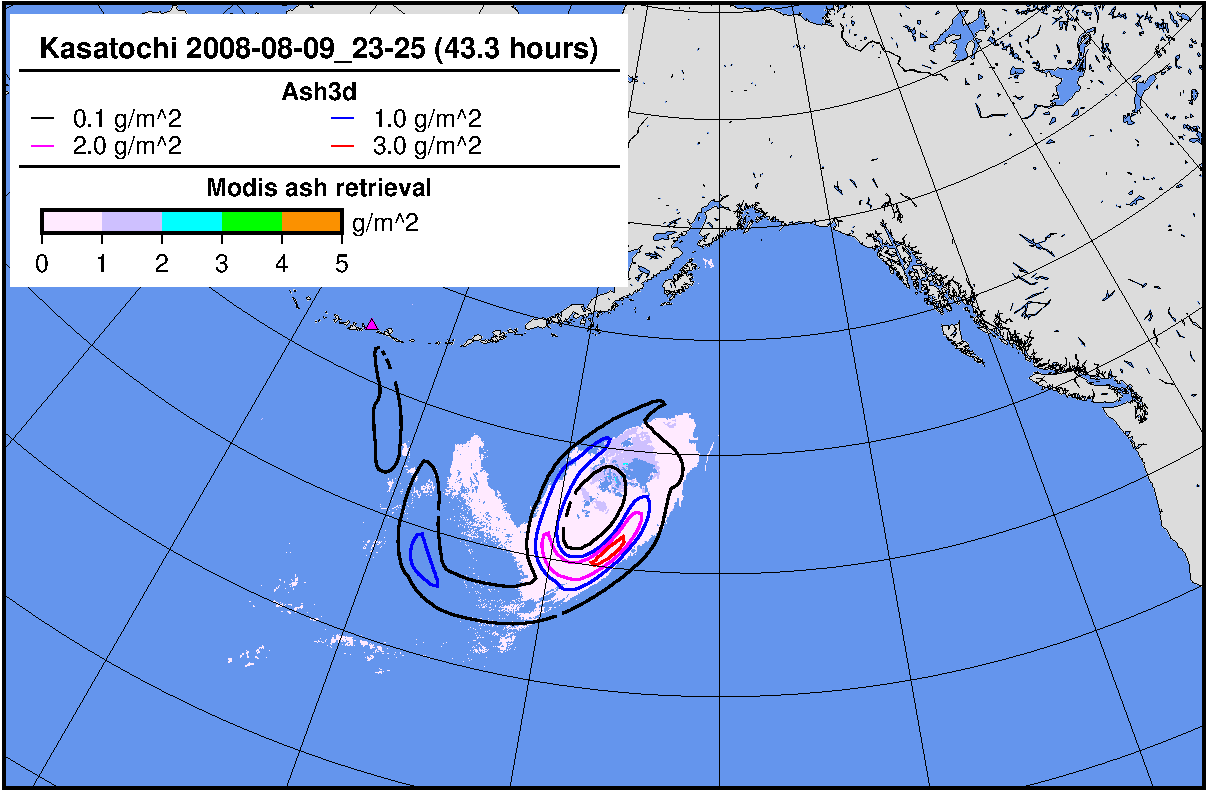
\includegraphics[angle=0,scale=0.3]{Figures/TestCase_Results/ValidTest/Kasatochi_CloudLoad_3.pdf}
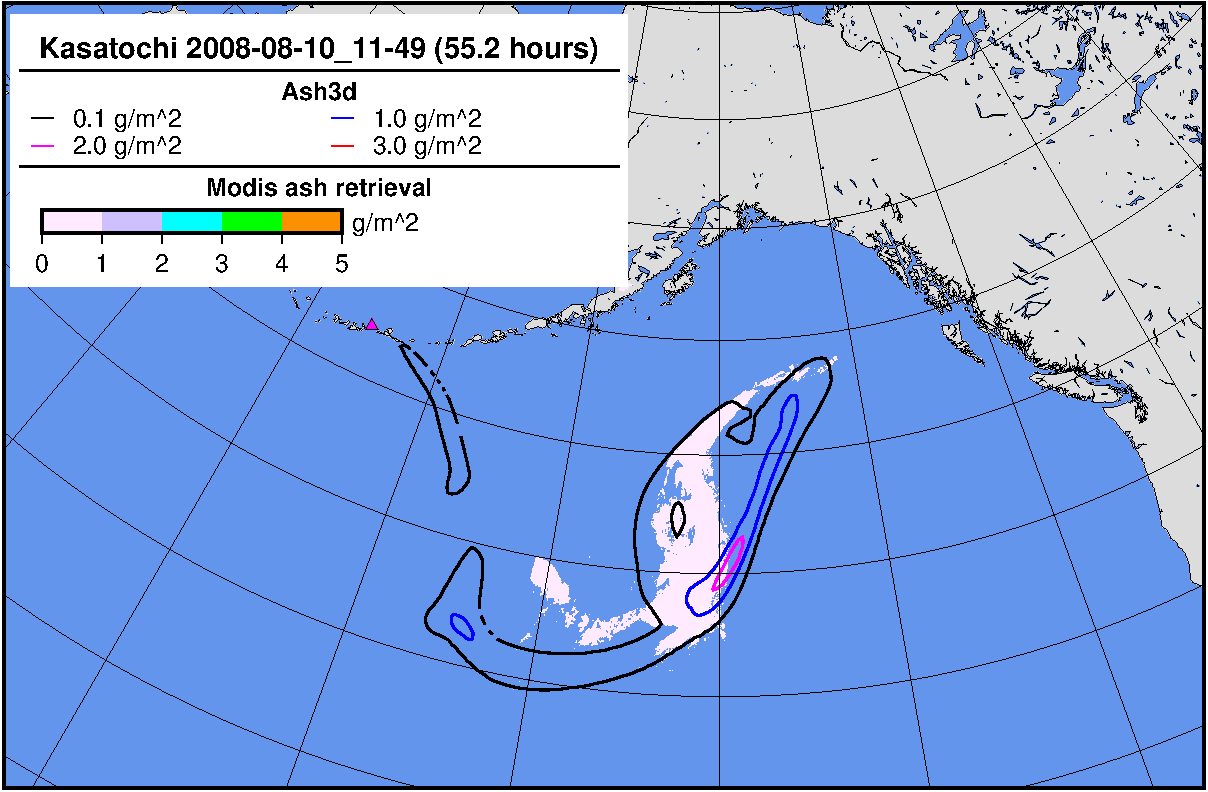
\includegraphics[angle=0,scale=0.3]{Figures/TestCase_Results/ValidTest/Kasatochi_CloudLoad_4.pdf}
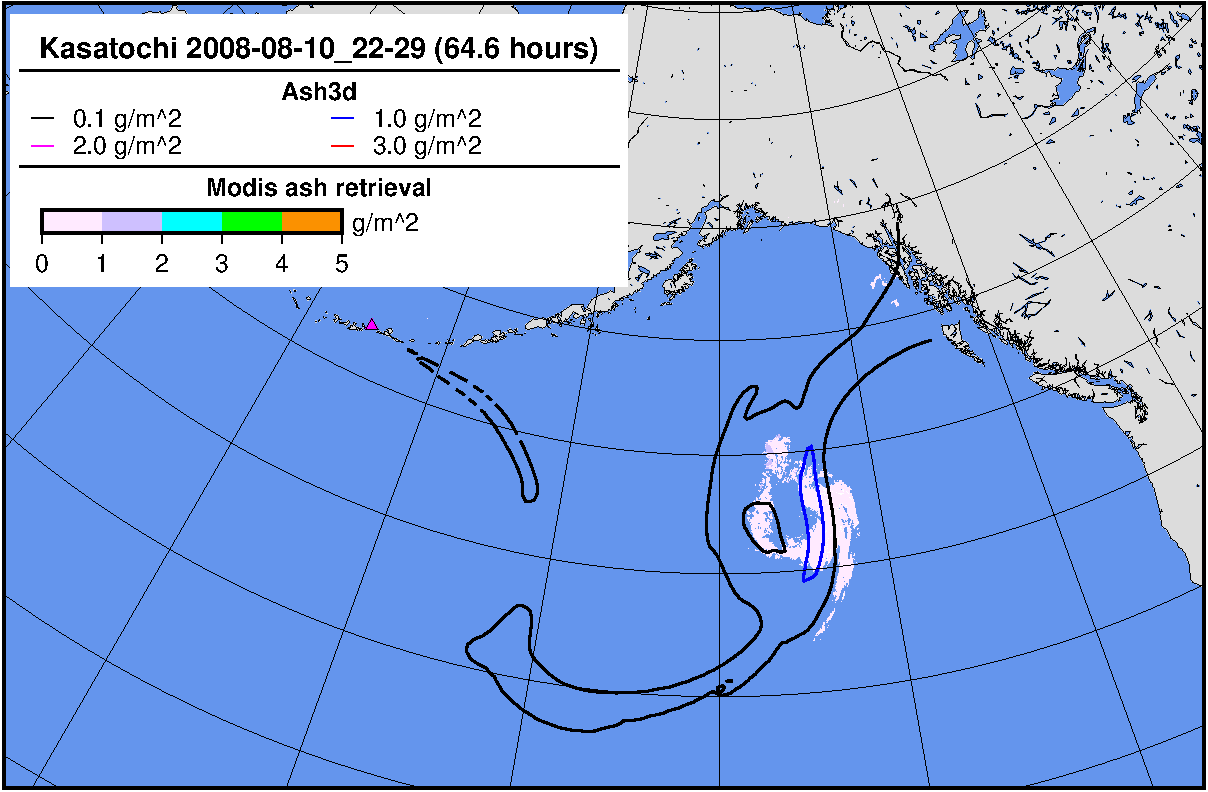
\includegraphics[angle=0,scale=0.3]{Figures/TestCase_Results/ValidTest/Kasatochi_CloudLoad_5.pdf}
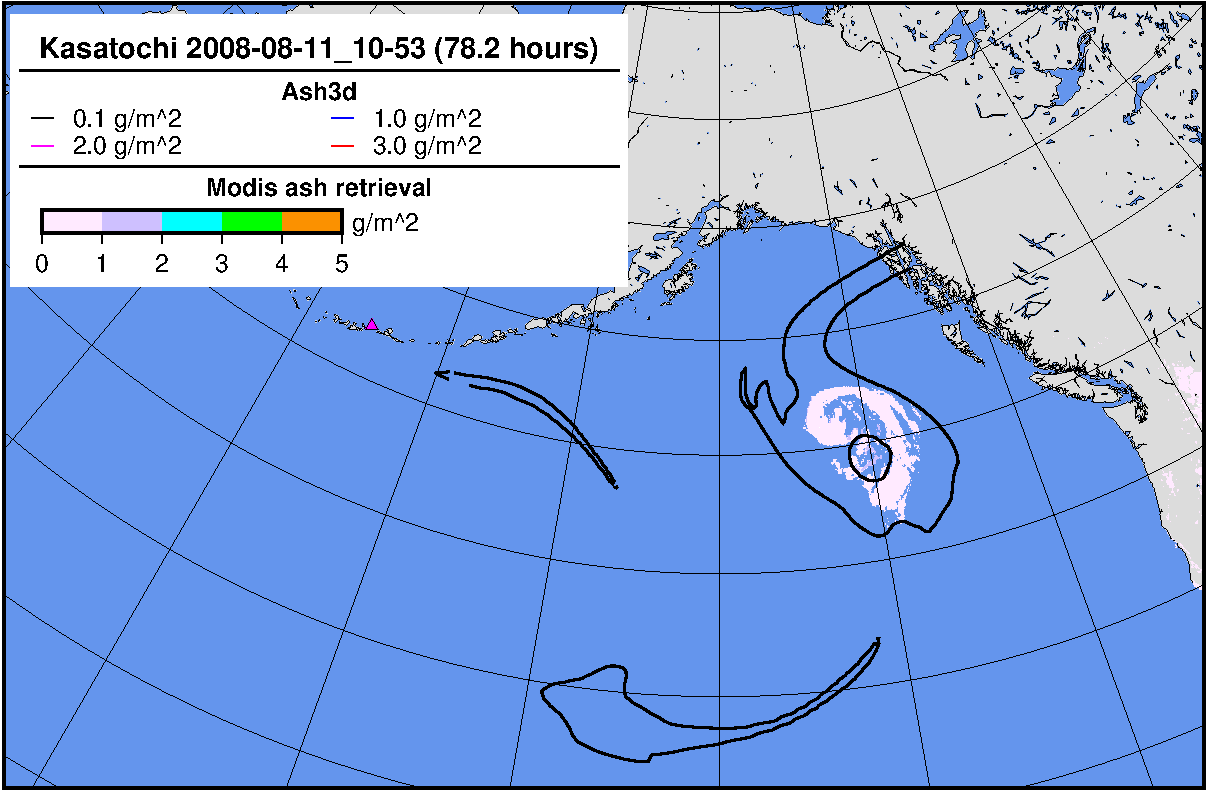
\includegraphics[angle=0,scale=0.3]{Figures/TestCase_Results/ValidTest/Kasatochi_CloudLoad_6.pdf}
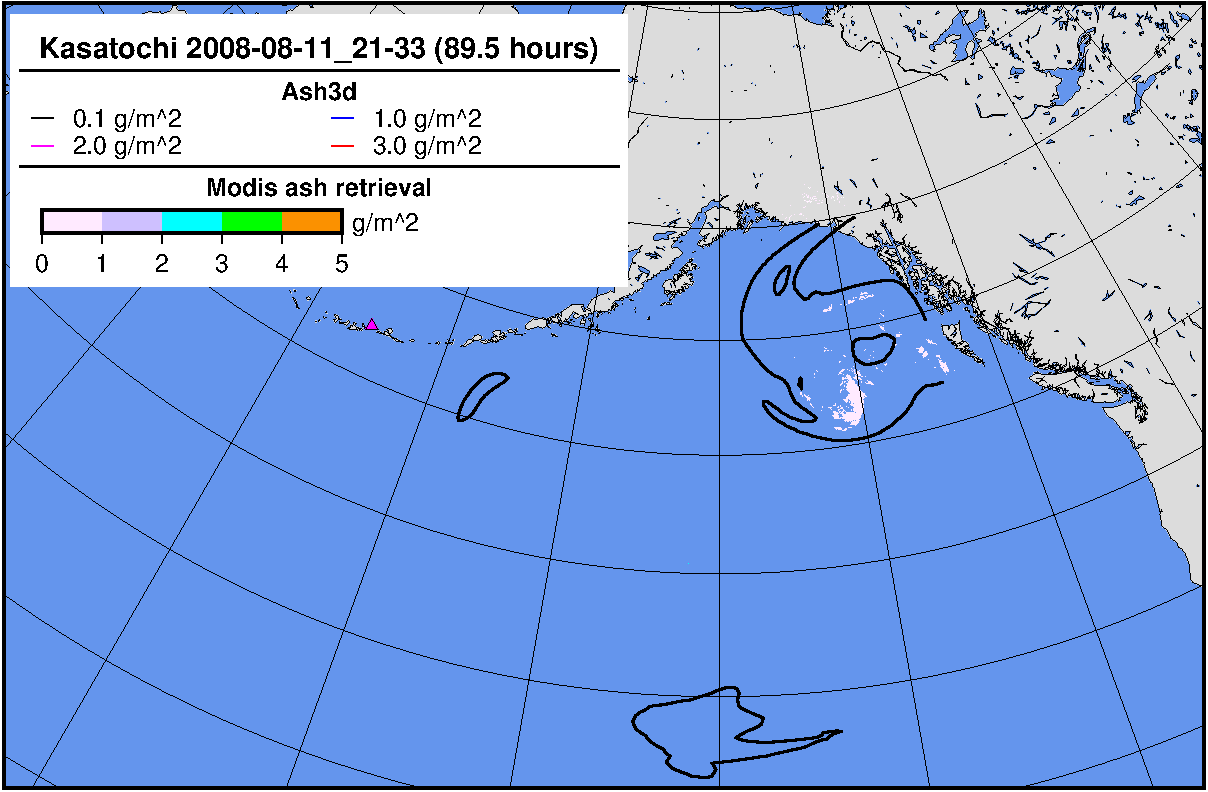
\includegraphics[angle=0,scale=0.3]{Figures/TestCase_Results/ValidTest/Kasatochi_CloudLoad_7.pdf}
\parbox{15cm}{\caption{\label{FigTestValKasatochi} Cloud load}}
\end{figure}

\clearpage
\subsection{Mazama (Deposit from Umbrella Source)}
\begin{figure}[htbp]
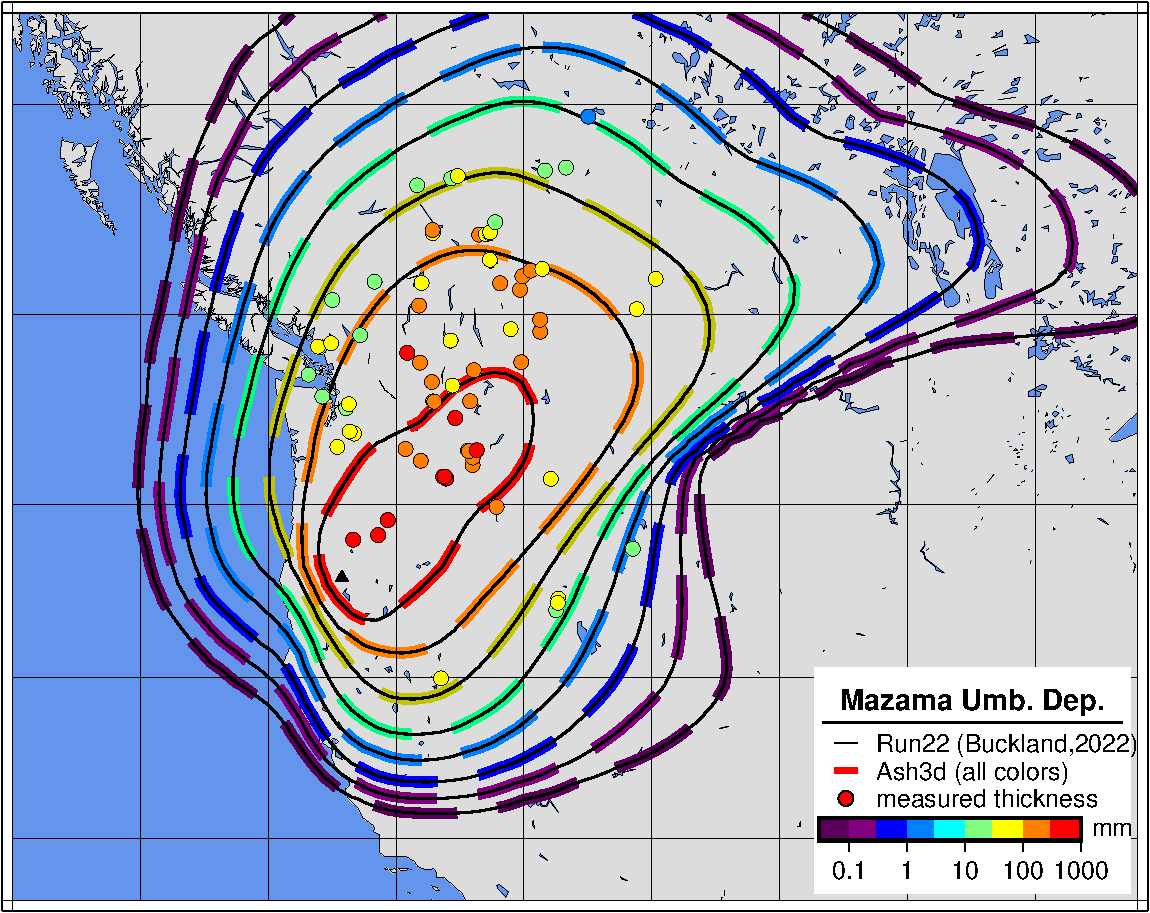
\includegraphics[angle=0,scale=0.6]{Figures/TestCase_Results/ValidTest/Mazama_UmbrellaDeposit.pdf}
\parbox{15cm}{\caption{\label{FigTestValMazama} Deposit}}
\end{figure}

\clearpage
\subsection{Kelud (Ash Cloud from Umbrella Source), Feb. 13, 2014}
\begin{figure}[htbp]
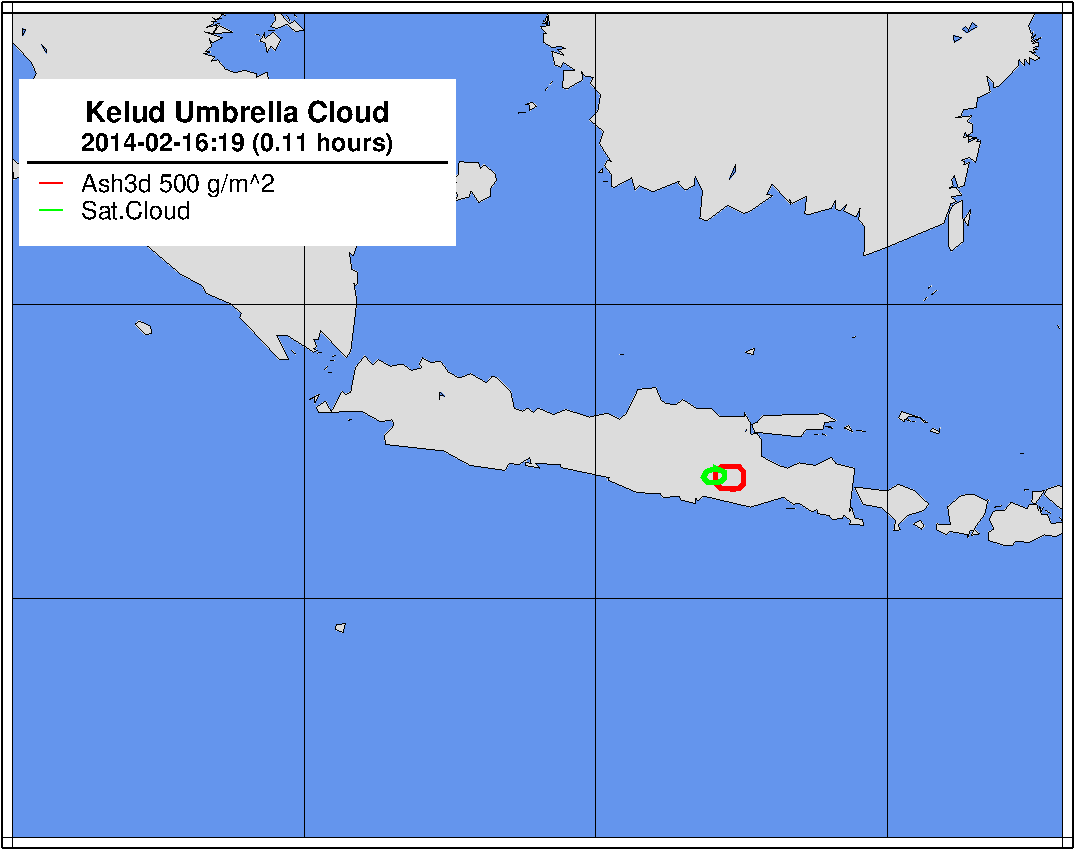
\includegraphics[angle=0,scale=0.3]{Figures/TestCase_Results/ValidTest/Kelud_CloudOutline_0.pdf}
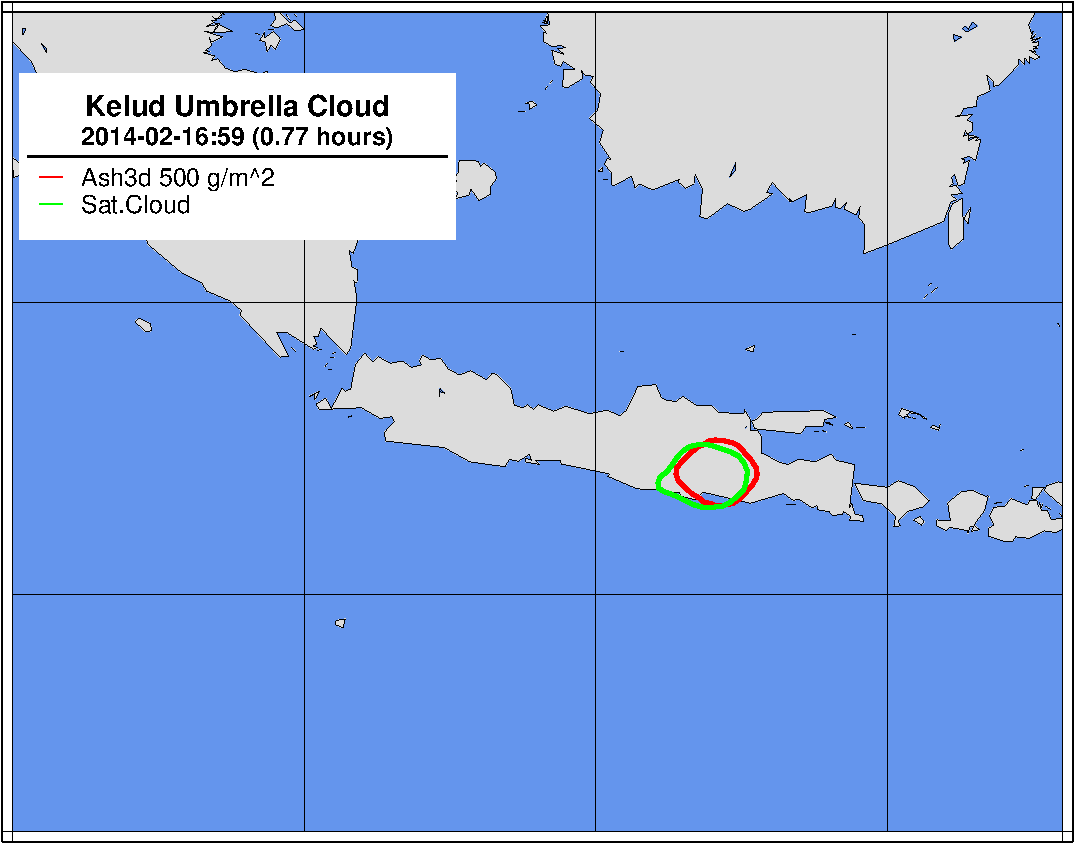
\includegraphics[angle=0,scale=0.3]{Figures/TestCase_Results/ValidTest/Kelud_CloudOutline_1.pdf}
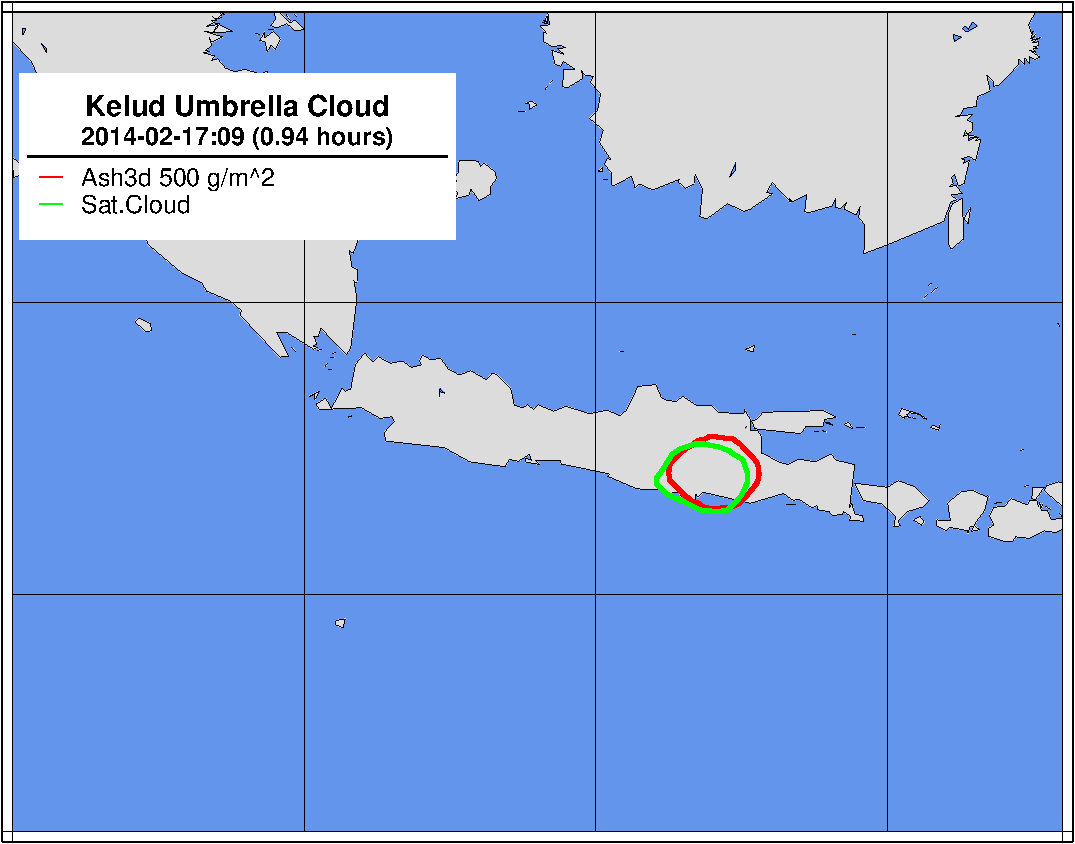
\includegraphics[angle=0,scale=0.3]{Figures/TestCase_Results/ValidTest/Kelud_CloudOutline_2.pdf}
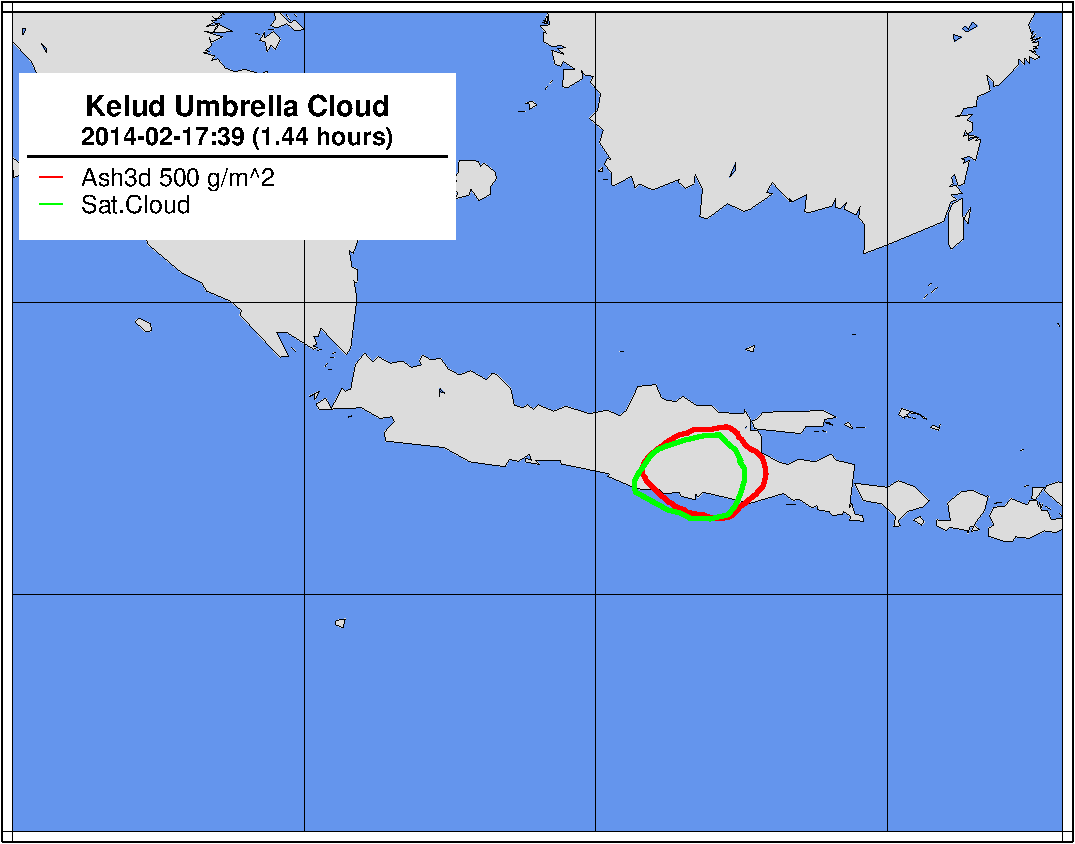
\includegraphics[angle=0,scale=0.3]{Figures/TestCase_Results/ValidTest/Kelud_CloudOutline_3.pdf}
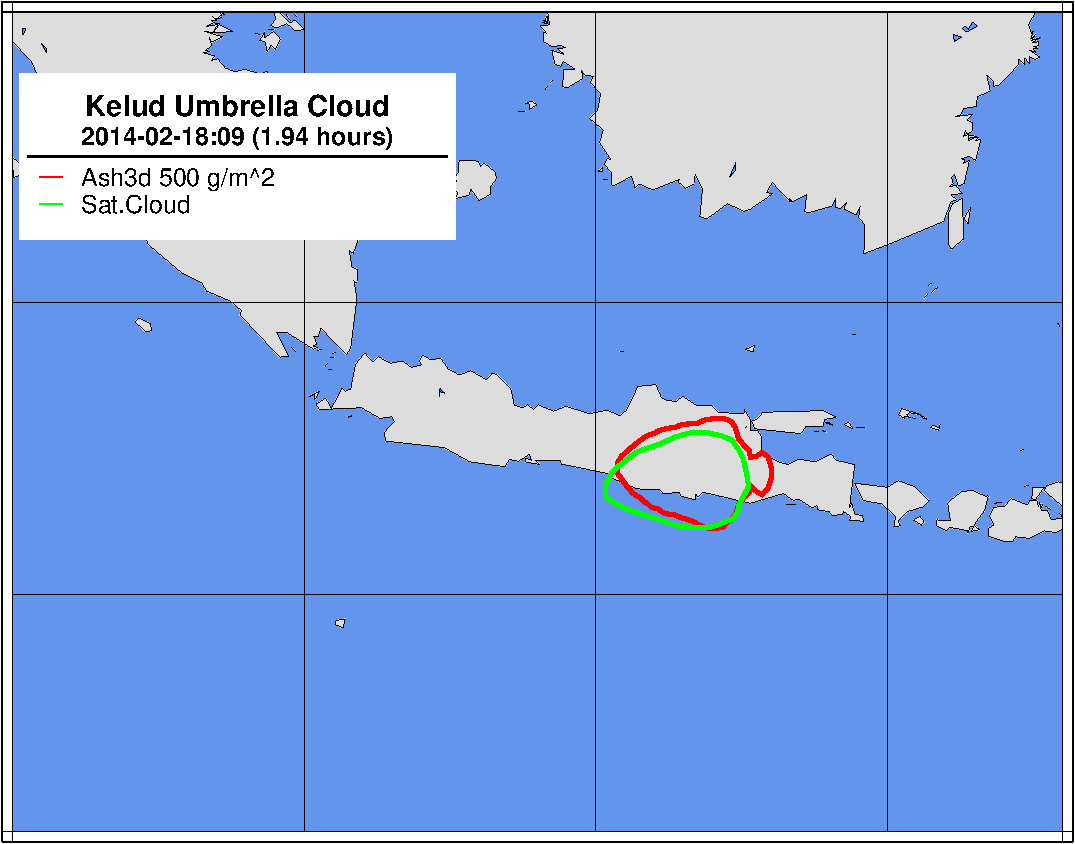
\includegraphics[angle=0,scale=0.3]{Figures/TestCase_Results/ValidTest/Kelud_CloudOutline_4.pdf}
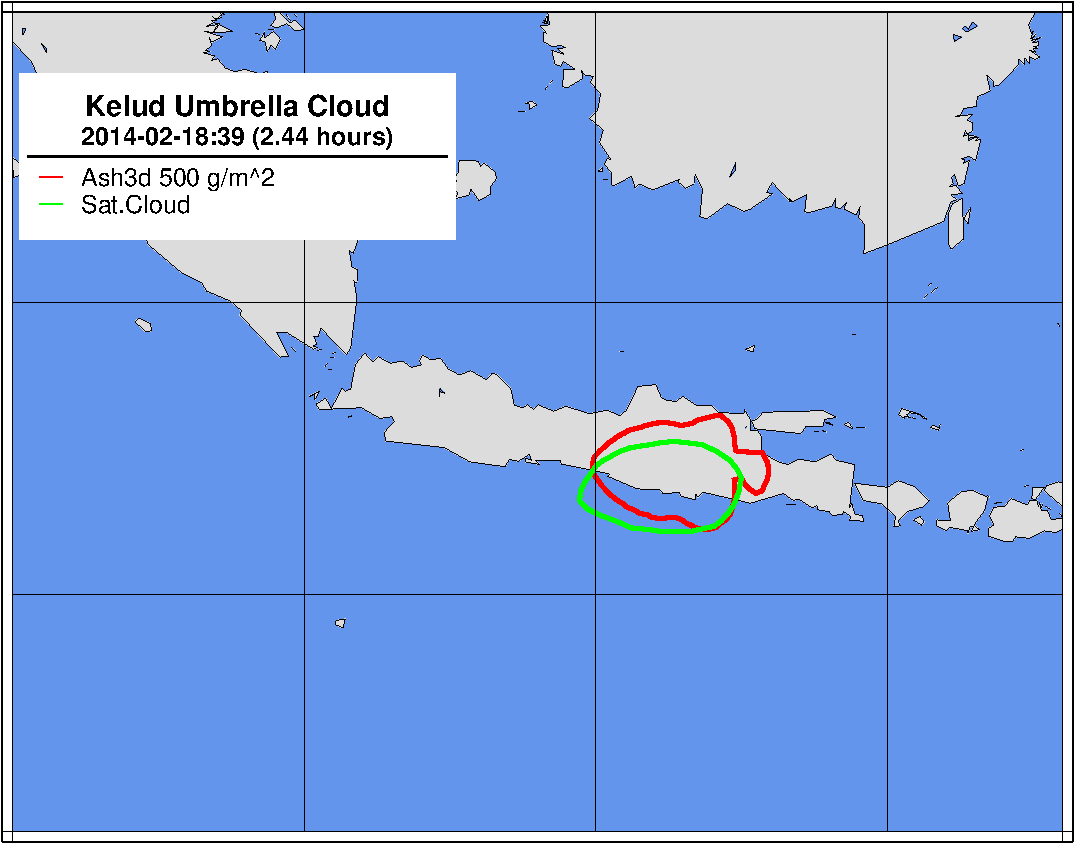
\includegraphics[angle=0,scale=0.3]{Figures/TestCase_Results/ValidTest/Kelud_CloudOutline_5.pdf}
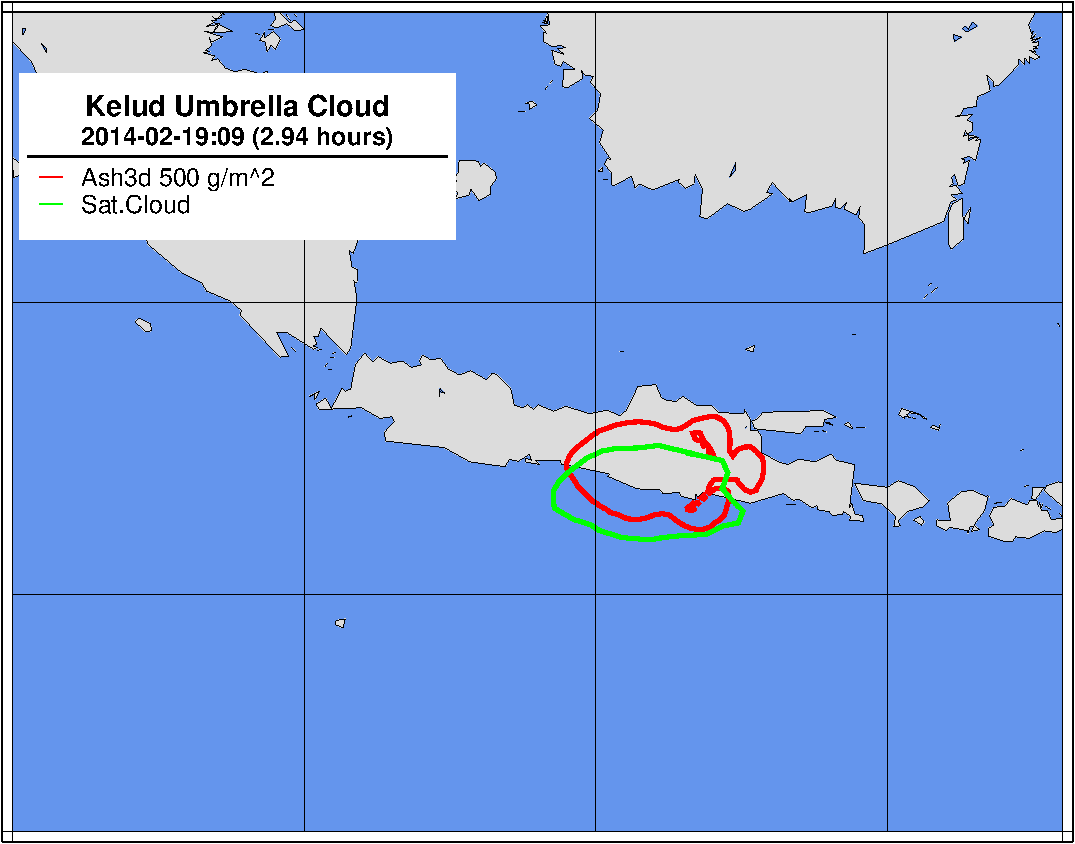
\includegraphics[angle=0,scale=0.3]{Figures/TestCase_Results/ValidTest/Kelud_CloudOutline_6.pdf}
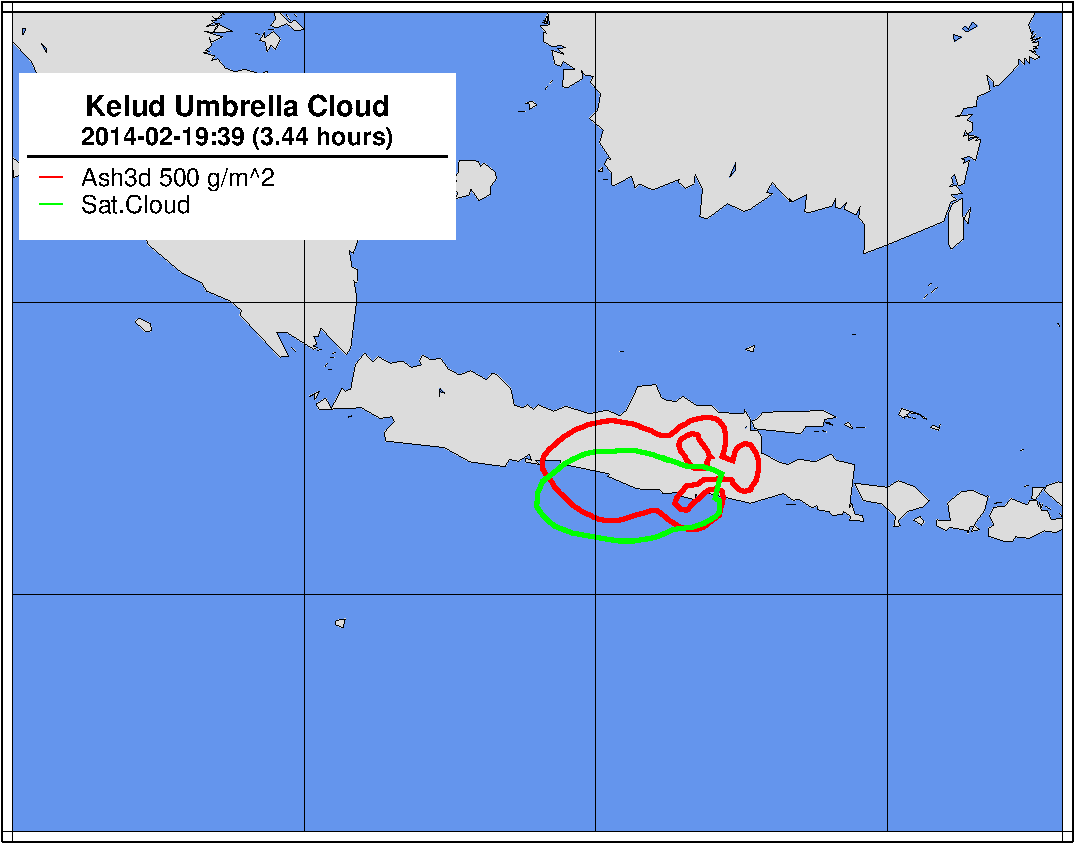
\includegraphics[angle=0,scale=0.3]{Figures/TestCase_Results/ValidTest/Kelud_CloudOutline_7.pdf}
\parbox{15cm}{\caption{\label{FigTestValKelud} Umbrella Cloud Spreading rate}}
\end{figure}

%\subsection{}

